As scalable information technology evolves to a more cloud-like model,
{\em digital assets} (code, data, software environments, and technologies) 
are increasingly integrated into applications by developers 
as web-accessible services.
This application development model facilitates code reuse and eases the 
assembly of complex systems thereby greatly improving programmer productivity
over non-service-oriented methodologies~\cite{Dan:2008:SSR:1370916.1370923}. 
By composing an application from existing services that 
encapsulate common yet complicated tasks such as
database access, logging, and security, or the audited access of useful 
digital assets, application developers are able  
to work at a higher level of abstraction, employ any programming 
language they choose, leverage the work, testing, and quality
assurance of others, and thus innovate faster.  

\begin{floatingfigure}[rb]{2.8in}
\vspace{-0.1in}
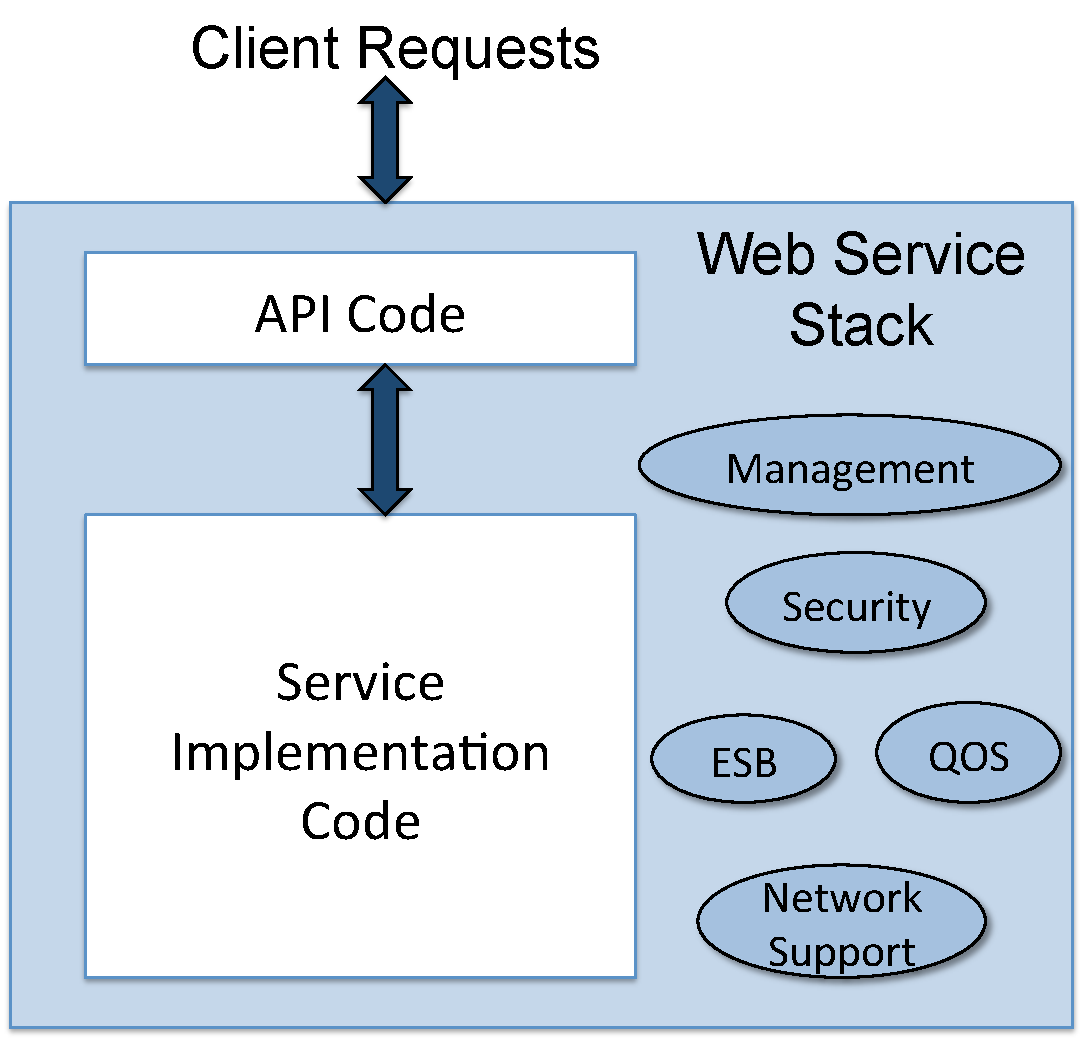
\includegraphics[scale=.34]{stack}
\vspace{-0.08in}
\caption{Web Service Software Components\label{fig:ws-arch}}
\end{floatingfigure}
Production web services consist of three components: API code, service
implementation code, and a web service ``stack'' that implements a container
for combining and deploying the API and service implementation
together ({\em c.f.} Figure~\ref{fig:ws-arch}).
Clients contact the web service container which routes requests to the
API code.  The container implements common functions such as 
service management (registration, description, discovery), a service
bus (ESB), security policy enforcement, and networking support, among other 
functions that both API and service implementation code access.
Service clients in production settings can be 
external, i.e., customers of the enterprise, or internal, i.e., employees of 
the organization.  These clients access the services via user 
interfaces (e.g. via a browser) or programmatically via web applications 
or other services. 

Increasingly, IT organizations are tasked with deploying and 
maintaining web services as software infrastructure components, hosted in a
shared cloud platform ({\em i.e.} in a way analogous to the manner in which they
would deploy and maintain a piece of shared physical infrastructure).  
To achieve economies of scale, these services are shared (in a controlled
way) among the widest possible set of users and client applications.  Indeed,
it is the possibility of Internet-scale sharing that makes this model
attractive from an IT management perspective. As a consequence we 
are witnessing an explosion of web APIs on the Internet today. ProgrammableWeb,
the popular online API registry currently boasts over 12,000 registered APIs and
a near exponential growth rate since 2006.

The modular design of web services inherently separates API, 
service implementation, and container. However, only 
the service implementation and the container is under complete
control of IT. External clients access APIs independently from IT.
Even internally developed client applications may be too numerous and
constantly evolving for IT to track or control given
potentially tens or hundreds of engineering teams and hundreds or 
thousands of APIs.  That is, the decoupling of the API from the 
other components of the web service provides many programmer
benefits, but it also introduces several IT management challenges 
at production scales. 

The confluence of application concerns ({\em e.g.} 
application functionality and productivity) with IT 
concerns ({\em e.g.} life cycle management, security, 
cost management) has led to new organizational approaches such as
DevOps.  However, 
the technologies that have been developed
to date address the core API
governance challenges incompletely, if at all. 
In particular, new research and technology is needed 
to provide scalable and unified automation to the problem
of implementing and enforcing consistent governance for APIs. 
By using automation to ensure consistency, our goal is to alleviate the 
labor burden associated with uniform policy implementation and SLA enforcement.  
Consistent policy implementation across APIs will reduce (and perhaps
eliminate) some of the cost scaling factors that the need for API governance
introduces.  Thus, at the same time automation ensures cost-saving
consistency, we believe it will also lead to productivity gains for 
IT management through reduced labor burden.

To my knowledge, there is no extant system that automates governance and
SLA enforcement across the life cycle
of an API, across diverse categories of policies, for web
APIs in cloud environments simply and scalably.  The goal of my work is to investigate 
new research and to develop
new technologies that do so for the next generation of service ecosystems.